\documentclass{beamer}
\usepackage[ngerman]{babel}
\usepackage[utf8]{inputenc}
\usepackage[T1]{fontenc}
\usepackage{textcomp}
\usepackage{graphicx}
\usepackage{subfiles}


\graphicspath{{resources/}}

\beamertemplatenavigationsymbolsempty

\title{Funktionale Programierung}
\subtitle{Concurrency \& Parallelism}
\author{Jan-Philipp Willem}
\institute{Hochschule Mannheim}
\date{SEM WS2016, \par Prof. Dr. Sandro Leuchter}



\begin{document}
\begin{frame}<handout:0>
  \frametitle{..?}
  \centering
  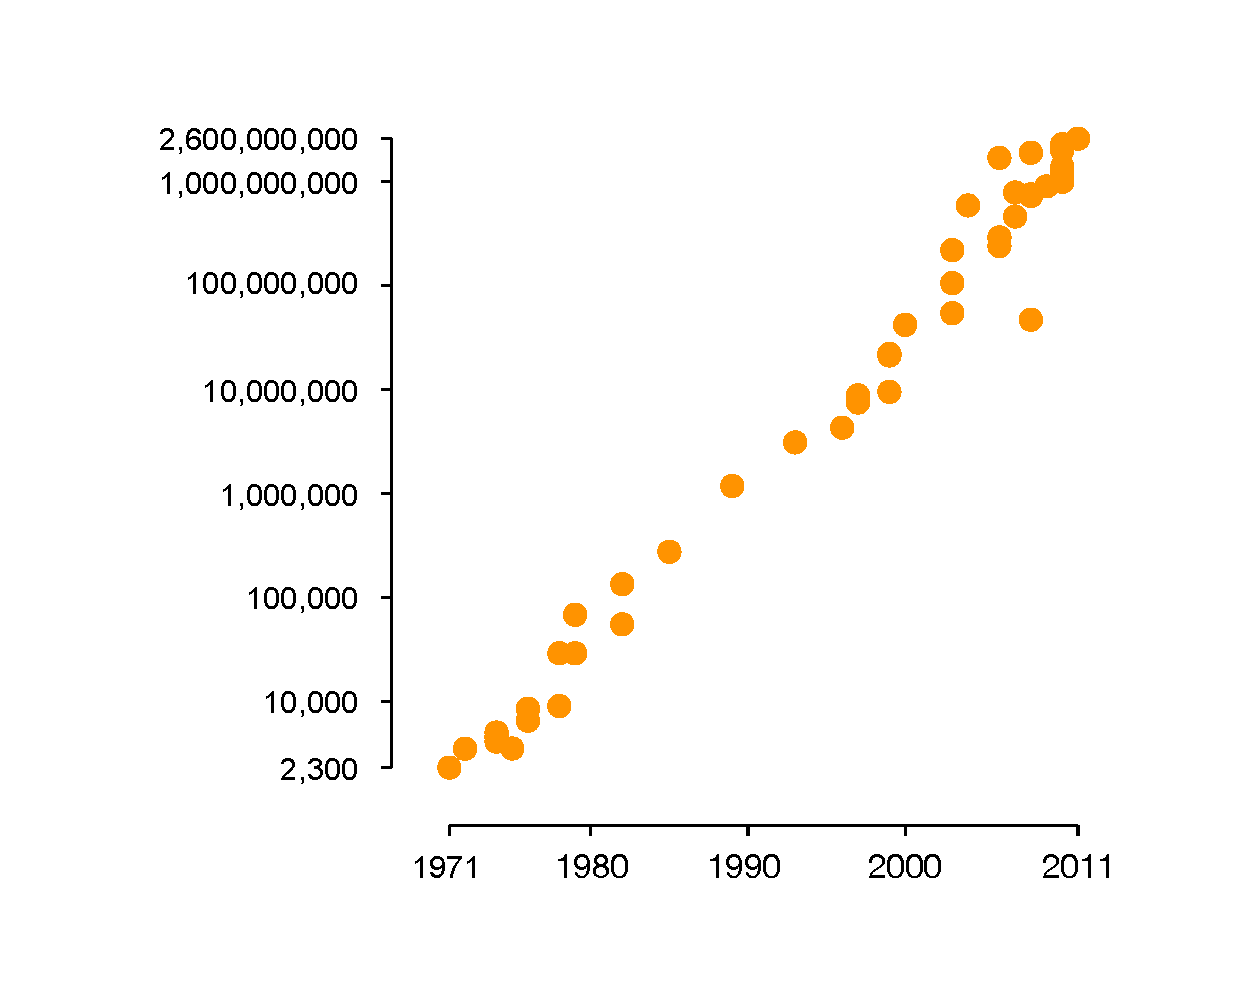
\includegraphics[width=1.0\textwidth]{moores_law.pdf}
\end{frame}
 
\begin{frame}
  \frametitle{Microprocessor Transistor Counts 1971-2011 \& Moore's Law}
  \centering
  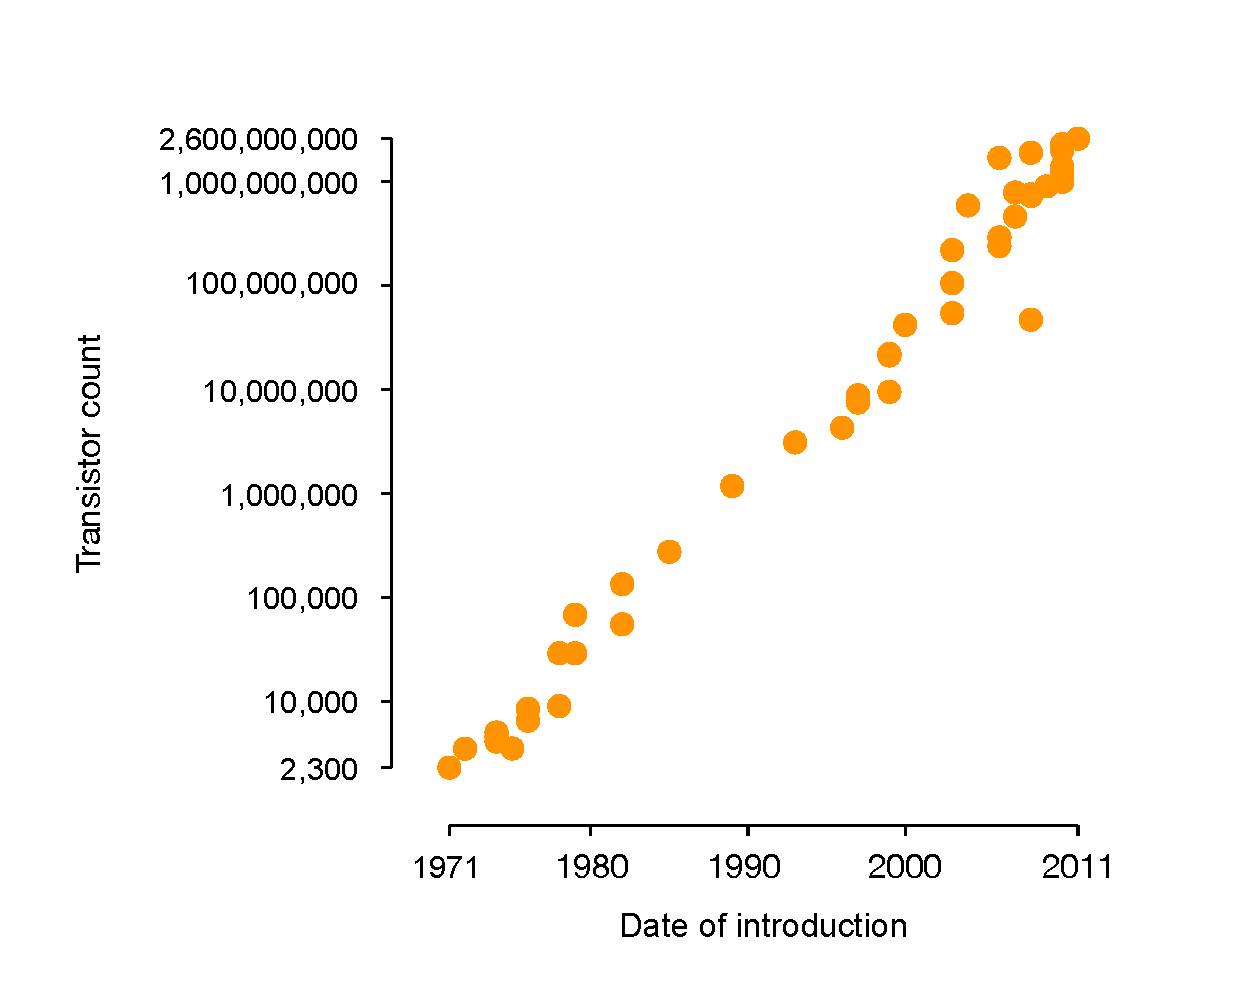
\includegraphics[width=1.0\textwidth]{moores_law_with-labels.pdf}
\end{frame}

\frame{\titlepage}

\begin{frame}
\frametitle{Table of Contents}
\tableofcontents
\end{frame}

\section[Bla]{Bla}
\begin{frame}
\frametitle{Sample frame title}
This is a text in first frame. This is a text in first frame. This is a text in first frame.
\end{frame}

\section[Foo]{Foo}
\begin{frame}
\frametitle{Sample frame title}
This is a text in first frame. This is a text in first frame. This is a text in first frame.
\end{frame}
\end{document}
